\chapter{Conversion to Mark}
\label{chap:ctm}

At this stage in the pipeline, we have tree edit distances $T_{i,j}$ where $i\in[0, N)$ $j\in[0,M)$ for $N$ student solutions and $M$ reference solutions. Our next step is to convert these edit distances into $N$ marks, one for each student. We are not aware of any established techniques for this process. As a result, we investigated several approaches based on our intuition (Section~\ref{sec:ctm-full-marks} to \ref{sec:ctm-clustering}) and presented our results in Section~\ref{sec:ctm-results}.

\section{Experiment Setup}

\subsection{Test Data}

We had student code and marks from 2017 and 2018 classes to analyze. Our plan was to use our tool to generate marks for these classes and compare our automated marks with human-evaluated marks (ground-truth).

\subsection{Cutoff Points}
\label{sec:ctm-cutoffs}

Recall that ClangAutoMarker's ultimate goal was to compute a student's mark, a value between 0 to 100, by comparing their solution's AST to the reference solution's AST. For a student to earn a full mark of 100 from our tool, the student would need to have structurally-identical code to the reference solution(s). However, this was essentially impossible unless the student had cheated in some form.

Assuming that students did not plagiarize current or past students, we erred on the side of caution and automatically rounded up our automated marks from a certain cutoff point. In our experiments, we tested cutoff points at 90 and 95. We chose these cutoff points from experience: in this range, the students were close enough to full marks that if they were from a human marker, the minor deductions resulting in a 90 or 95 might have essentially been due to the marker's mood and how lenient they were with minor issues. However any marks lower than 90 from a human marker were very likely to be indicative of actual errors in the student program.

We used the following formula to compute the students' final marks. To avoid confusion, we shall henceforth denote the final value to be returned to the student as \textquote{Mark} and denote the computed value from our methods in Sections~\ref{sec:ctm-full-marks} to \ref{sec:ctm-clustering} as \textquote{Score}. 

\[
  \text{Mark}_i =
  \begin{cases}
    \text{Score}_i & \text{if Score$_i$ $<$ Cutoff} \\
    100            & \text{if Score$_i$ $\geq$ Cutoff}
  \end{cases}
\]

\subsection{Effectiveness}

We measured the effectiveness of ClangAutoMarker by counting how many assignments it could successfully automate, i.e. scored above the cutoff points of 90 or 95. Conversely, an assignment must be manually reviewed if we were uncertain about the mark we generated, i.e. scored below 90 or 95. There were two cases where this could happen.

The first case was if the student code had non-conventional coding patterns. It is likely that there will be a few outlier students in every class who write their code significantly different than what we normally expect in our reference solutions. Even if their solution was functionally correct, their AST would have an extremely high edit distance from our reference solutions and thus would receive an undeserved low score.

The second case was if the student program cannot be processed by our tool. This occurred if the student had syntactical errors or if the student's AST deviated from one of our assumptions and triggered an internal assertion error. For example, we assumed that all solution files have a \texttt{main} function; if this function was missing then we would not be able to perform any of our analyses and thus would require manual intervention.

To capture both cases, we designated an assignment for manual review if its score was too low or non-existent (e.g. process ended early due to assertion error). For the sake of simplicity, we deemed an automated score to be too low and thus require manual review if it was below the cutoff points previously mentioned.

\subsection{Accuracy and False Positives}

Out of the assignments that our tool could automate, we evaluated the accuracy or false positive rate of our accepted predictions. We designated an assignment to be a false positive if its mark (not the same as score) was significantly higher than what a human marker assigned to it. In practice, we tolerated an excess of up to 10 points before we considered a mark to be a false positive because, as discussed in Section~\ref{sec:ctm-cutoffs}, human markers generally could vary their evaluation by up to 10 points for trivial issues.

It is important to note that the marks we used as ground-truth also included a written report. Furthermore, our ground-truth marks also contained deductions from non-technical issues such as late submissions or plagiarism. Unfortunately, detailed historical data were not kept after the course ended. Since these unrelated deductions were included in our ground-truth, our real false positive rate might actually be lower than what we present.

\section{Always Full Marks}
\label{sec:ctm-full-marks}

Since we expected most of the class to receive full marks for the assignment, we used the trivial approach of always giving everyone full marks as our baseline to measure the accuracy and effectiveness of our other approaches. Any other marking technique must perform better than this \textquote{automatic} technique to be considered an improvement over manual marking.

\section{Minimum Distance}

We used multiple reference solutions to cover the various approaches to solving their respective assignments. A correct student solution should closely match at least one of these reference solutions and thus have an extremely small edit distance from it. Therefore, we initially assumed the student's mark should be based on the smallest edit distance to reference solutions.

Since our cost model assigned an absolute value instead of relative difference, it was impractical to compare the actual edit distance between each reference solution. Therefore, we needed to first normalize the edit distances before we could properly compare how close a student solution is to other reference solutions.

There are many approaches to normalizing values; we chose to use the MaxAbsScaler algorithm in the Sklearn Python library \cite{MaxAbsScaler} because we believed it was the most suitable one for our purpose. For reference solution $j$, the algorithm normalized its edit distance to each student $T_{1,j}, T_{2,j}, \ldots, T_{N,j}$ to be between 0 and 1. This algorithm also did not shift the data and was thus able to preserve the relative distances between students.

After normalizing student $i$'s edit distances to each of the $M$ reference solutions, we calculated the student's score as follows:
\begin{equation*}
\text{Score}_i = 100 \cdot (1 - \min \{ T_{i,1}, T_{i,2}, \ldots, T_{i,M} \})
\end{equation*}

\section{Clustering}
\label{sec:ctm-clustering}

The next idea we attempted was using clustering algorithms to group student solutions together. The goal was to put student solutions with similar edit distances, to some subset of reference solutions, in the same cluster.

Under this mindset, we treated each student as an independent \textquote{data point} and their edit distance to each reference solution as an independent \textquote{feature}. Our data thus became an $N \times M$ matrix with $N$ rows for each student and $M$ columns for each reference solution.

We made the assumption that full-mark solutions should have very similar features and thus should be very close to each other in the same cluster. Recall that the majority of the historical student solutions in this course had received full marks. Therefore, the majority of each cluster's points should also be very close to each other as well. As a result, we believed each cluster should theoretically be \textquote{centered} closer to the full-mark solutions than the incorrect solutions; therefore we hypothesized the closer a student solution was to the cluster's center, the higher the probability that the student solution should receive full marks.

%------------------------------------------------------------------------------
\subsubsection{Determining Number of Clusters}
%------------------------------------------------------------------------------

The K-Means and Gaussian Mixture clustering algorithms require us to specify how many clusters we want to find in our data points (student solutions). There are no straightforward approaches to choosing this value because it depends on the input data and use-case.

If we choose too few clusters, then we risk putting too many student solutions in the same cluster despite them not being too closely related. If we choose too many clusters, then we risk not getting sufficient data to compute scores. For example, in the extreme case of $N$ clusters, every student would become its own cluster and, according to our original hypothesis of final score being based on closeness to a cluster's center, should receive full marks.

However, there are techniques such as the \textquote{Elbow Method} \cite{thorndike1953belongs} shown in Figure~\ref{fig:ctm-num-clusters} that can be used for guidance. For our data, the Elbow Method recommended for us to use 4 clusters.

\begin{figure}
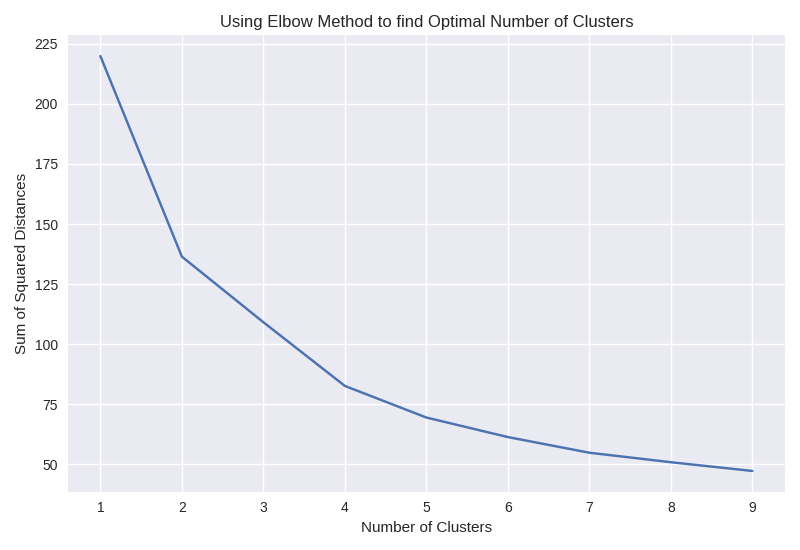
\includegraphics[width=\textwidth]{elbow}
\caption[Using Elbow Method to find Optimal Number of Clusters]{The Elbow Method runs the K-Means clustering algorithm with a range of clusters and computes the sum of squared errors. This sum measures how close the predicted clusters match the data points; the greater the error, the less clusters fit the data. This graph converges to 0 at $N$ clusters where each point is its own cluster and thus has zero error. To find an appropriate number of clusters, we need to visually find an \textquote{elbow} point on the graph, i.e. where adding an additional cluster will not significantly reduce the error. In this graph, the elbow point is at 4 clusters.}
\label{fig:ctm-num-clusters}
\end{figure}

%------------------------------------------------------------------------------
\subsubsection{Cleaning Up Data}
%------------------------------------------------------------------------------

Although not essential, we chose to perform Principal Component Analysis (PCA) \cite{wold1987principal} on our data prior to clustering. PCA transforms our set of $M$ features into a smaller set of linearly uncorrelated features or \textquote{components}. The components are sorted in descending order of variance. In other words, the first few components theoretically capture the majority of the \textquote{information} in the source data.

The most obvious advantage of PCA is reducing the runtime of our clustering algorithms because it eliminates features (columns in our data matrix) that represent very little information about our data points. This technique is also useful in visualization as it allows high-dimensional data to be presented in a 2D graph while preserving the majority of the information and relationships between data points.

To use PCA, we need to specify how many components or features to keep. Similar to the Elbow Method to determine the number of clusters, we can look at the graph of cumulative explained variance shown in Figure~\ref{fig:ctm-num-components} to estimate an appropriate number of components. For our data, the graph recommended for us to use 6 components.

\begin{figure}
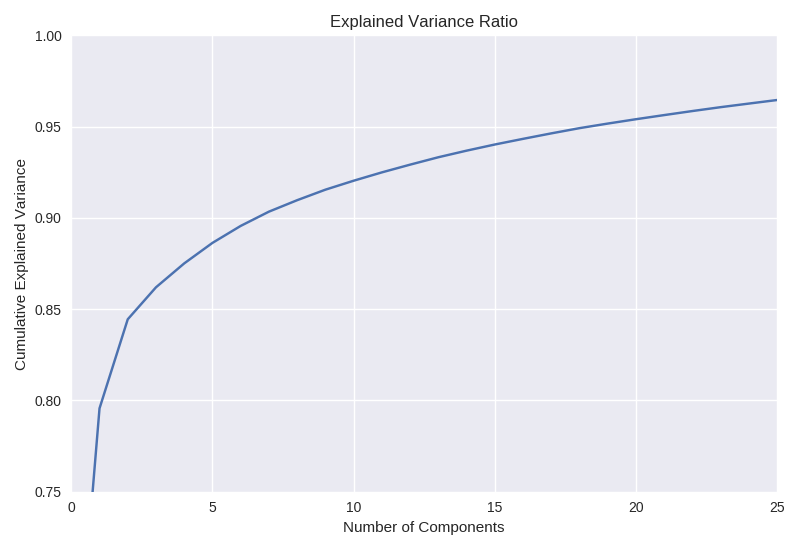
\includegraphics[width=\textwidth]{explained_variance_ratio}
\caption[Explained Variance Ratio]{The explained variance conceptually represents the amount of information in the original data that each component captures. The first component captures almost 80\% of the original information; the second component captures another 5\%; and so on. This graph show the cumulative explained variance that each additional component captures. A rule-of-thumb for PCA is to choose the number of components at an \textquote{elbow point} where adding an additional component will not capture significantly more information. In this graph, the elbow point is at 6 components.}
\label{fig:ctm-num-components}
\end{figure}

\subsection{K-Means}
\label{sec:ctm-km}

The first clustering algorithm we tried was K-Means \cite{macqueen1967some}. It iteratively tries to group unlabeled data points with similar features together by minimizing the mean distance between each point in each group. Figure~\ref{fig:ctm-km} visualizes the groups labeled by the K-Means algorithm on the 2017 class for the Non-Blocking IO assignment.

The K-Means algorithm constructs each group to minimize the average distance from the group's centroid to every point in its corresponding group. Since the majority of students in our data set received full marks, we assumed the majority of the data points in each group should also represent full-mark solutions. As a result, the volume of full-mark solution points should draw the centroid of each group towards \textquote{regions} representing higher marks. Based on this idea, we calculated a student's score based on their distance to their corresponding group's centroid; the closer a student was to their group's centroid, the higher their probability of receiving a high score.

Let $P_i$ denote the point representing student $i$ and $C_i$ denote the centroid of the student's group. The distance from centroid $d_i$ is defined as:
\begin{equation*}
d_i = \norm{P_i - C_i}
\end{equation*}

As mentioned in Figure~\ref{fig:ctm-km}, the scales in the axes have no tangible interpretations. Therefore, the distances from centroid $d_i$ we calculated for each point also had no meaningful interpretation. As a result, we tried to evaluate each point's centroid distance relative to all other points. In other words, we calculated each student's score based on their performance relative to the rest of their class.

Let $\mu$ denote the mean and $\sigma$ denote the standard deviation of centroid distances of every student. We calculated student $i$'s score as follows:
\begin{equation*}
\text{Score}_i = 100 - 20 \cdot \frac{\abs{d_i - \mu}}{\sigma}
\end{equation*}

This equation deducted up to 20 points for each standard deviation of centroid distance a student was from their corresponding group's centroid. We chose to deduct 20 points per standard deviation arbitrarily after experimenting with different values. The main idea was to deduct marks based on how far the solution was from the centroid, where we assumed majority of the full mark solutions were located.

\begin{figure}
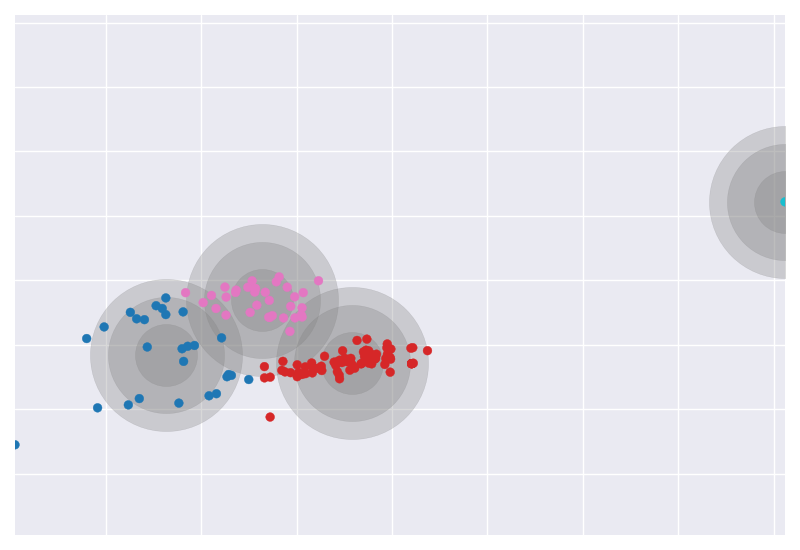
\includegraphics[width=\textwidth]{conversion-to-mark/marking_paster_nbio_ece459-a1-w2017_km}
\caption[K-Means Clustering]{Each data point represents a student solution to the Non-Blocking IO assignment from the 2017 class. It is important to note that this is a 2D projection of a multidimensional data set. Since we preprocessed the data with PCA, the first two dimensions presented here already capture the majority of the data variance. The scales in the axes are omitted because they have no tangible interpretations; they are meant for interpreting relative distances. The K-Means algorithm assigned each point a group, represented by their corresponding colour. Each set of concentric circles represent an arbitrary distance from the centroid of each group.}
\label{fig:ctm-km}
\end{figure}

\subsection{Gaussian Mixture}
\label{sec:ctm-gm}

The second clustering algorithm we tried was Gaussian Mixture \cite{dempster1977maximum}. Similar to the K-Means algorithm, it also groups unlabeled data points but with different criteria. As its name suggests, it assumes the points are randomly distributed following a Gaussian distribution. It iteratively tries to assign groups to maximize the likelihood of each data point belonging to their assigned groups. Likewise, we hypothesized that the closer a point (student solution) is to the centroid, in this case the central probability contour, the higher the probability of the student receiving a high score. In practice, we designated each student's score to be equal to the probability of them belonging to their assigned cluster, returned from the Gaussian Mixture algorithm.

\begin{figure}
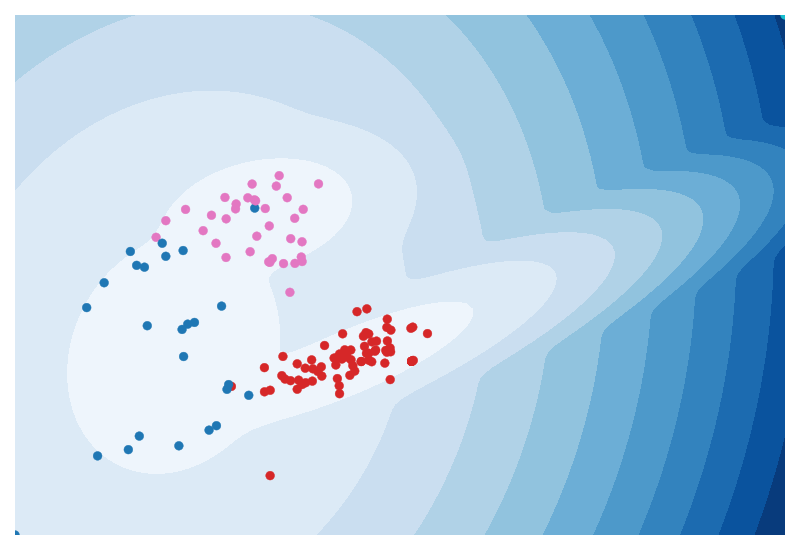
\includegraphics[width=\textwidth]{conversion-to-mark/marking_paster_nbio_ece459-a1-w2017_gm}
\caption[Gaussian Mixture Clustering]{This is a probability contour graph of our data points grouped by the Gaussian Mixture algorithm. Points closer to the center of the contours, i.e. lighter areas, have a higher probability of belonging to their corresponding group.}
\label{fig:ctm-gm}
\end{figure}

\subsection{HDBSCAN}
\label{sec:ctm-hdb}

The third and last clustering algorithm we experimented with was HDBSCAN (Hierarchical Density-Based Spatial Clustering of Applications with Noise) \cite{McInnes2017}. Similar to the previous two algorithms, it tries to group unlabeled data points with its own set of criteria. As its name implies, it tries to group points based on spatial density to ensure the resulting groups meet some density parameter.

The advantage of HDBSCAN is that it does not require us to specify the number of clusters we want to find. Instead, we specify the minimum number of points in each cluster $P$ and the algorithm will dynamically group points such that the resulting clusters have at least $P$ points. This gives us more flexibility in our parameters because choosing the number of clusters is harder than choosing the minimum number of points per cluster. We do not know the proper the number of clusters and thus must estimate it through an ad-hoc procedure. However, we do have a stronger conceptual understanding of the number of points per cluster: since we know there are only a limited number of approaches to solve an assignment and we know the majority of the students will follow similar approaches, either through collaboration or coincidence due to limited unique approaches, we know the $P$ value must be a significant fraction of the total number of students.

However, the disadvantage of this algorithm is that it is not guaranteed to be able to label every point; outlier points that cannot satisfy the group's density criteria are discarded as noise. The higher the minimum cluster size parameter $P$, the more points will be unlabeled. Ideally we want our groups to be as dense as possible so that we know the grouped points are extremely similar to each other. Ultimately, it is a balance between how many points we can label (automation rate) and how dense the resulting groups are.

Figure~\ref{fig:ctm-hdb} shows how the algorithm labels our data set based on varying minimum cluster sizes. A cluster size of 5 is able to achieve 3 groups, which is close to the 4 groups set for the previous two algorithms. However as we can see from the graph, the 3 groups are slightly sparse. As a result, we chose $P=10$ because it is able to label most of the points without sacrificing too much density; at higher cluster sizes, we do not seem to significantly increase our groups' densities.

Once we were satisfied with our parameters, we ran the HDBSCAN algorithm and designated each student's score to be equal to the \textquote{strength} of the student's corresponding group prediction returned from the algorithm.

\begin{figure}
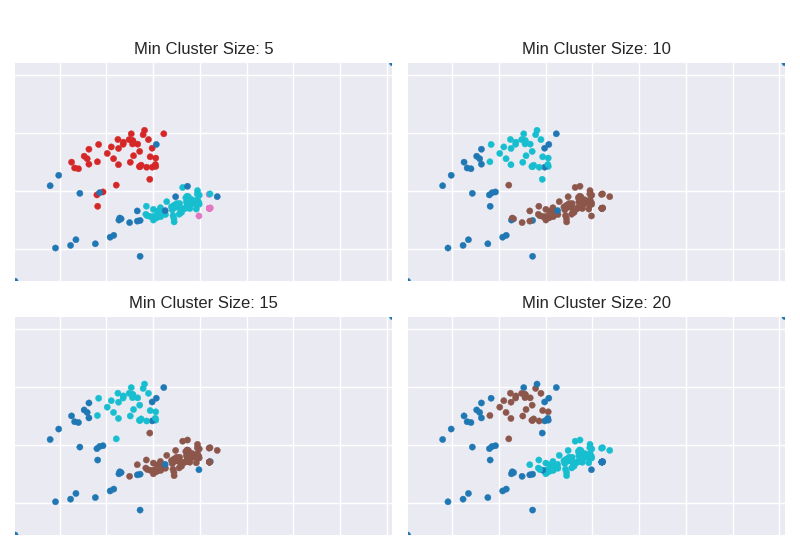
\includegraphics[width=\textwidth]{conversion-to-mark/marking_paster_nbio_ece459-a1-w2017_hdb}
\caption[HDBSCAN Clustering]{These graphs show our data points clustered with HDBSCAN using different minimum cluster size parameters. The higher the minimum size, the denser the resulting clusters. Furthermore, higher cluster sizes also result in more outlier points marked as noise (dark blue) as well as fewer total clusters. Cluster size of 5 has three different groups whereas cluster sizes of 10 and higher only have two different groups.}
\label{fig:ctm-hdb}
\end{figure}


%------------------------------------------------------------------------------
\section{Experimental Results}
\label{sec:ctm-results}
%------------------------------------------------------------------------------

Before we present our results, we will first discuss the possible outcomes from our tool in Table~\ref{tab:ctm-possible-outcomes}. Recall that we round up the predicted scores from our algorithms if the student scores above certain cutoff points. After rounding, we check if their true mark from historical data is within 10 points of 100 (to account of variance in human marker leniency). Ideally, we would like to cover the full range of marks. However because our tool does not provide meaningful feedback for deductions, other than the fact that the student's solution structure was notably different from our reference solutions, we decided to focus our efforts on optimizing the accuracy for scores above cutoff points. As a result, our tool's purpose essentially becomes \textquote{flagging} correct solutions; any solutions not flagged will be designated for manual marking.

Ultimately, we would like to maximize the number of predicted scores above cutoff points while minimizing the number of false positives. The more assignments that are predicted to score above our cutoffs, the less manual work will be required from human markers. While most students would not complain about undeservedly receiving full marks, too many false positives (and student knowledge thereof) would diminish the formative value of the assignments. That is, if students were aware of a high false positive rate due to assigning full marks, we are concerned about complacency or apathy towards completing their assignments.

\begin{table}
\definecolor{lgray}{gray}{0.75}
\begin{tabular}{l!{\color{lgray}\vrule}l!{\color{black}\vrule}cc}
\Toprule
\multicolumn{2}{c!{\color{black}\vrule}}{} & \multicolumn{2}{c}{True Mark} \\ \arrayrulecolor{lgray}\cline{3-4}\arrayrulecolor{black}
\multicolumn{2}{c!{\color{black}\vrule}}{} & $<$ 90 & $\geq$ 90 \\
\Midrule
\multirowcell{2}{Automated\\Score} & $<$ Cutoff    & Correct Prediction & False Negative \\
                                   & $\geq$ Cutoff & False Positive     & Correct Prediction \\
\Bottomrule
\end{tabular}


\caption[Possible Outcomes for ClangAutoMarker Predictions]{This table presents the possible outcomes from our tool's predictions. Without meaningful feedback for deductions, only automated scores above our cutoff points (which will later be rounded up to full marks) are relevant for us. As a result, the relevant outcomes for our tool lie in the bottom row of this table.}
\label{tab:ctm-possible-outcomes}
\end{table}

\begin{figure}
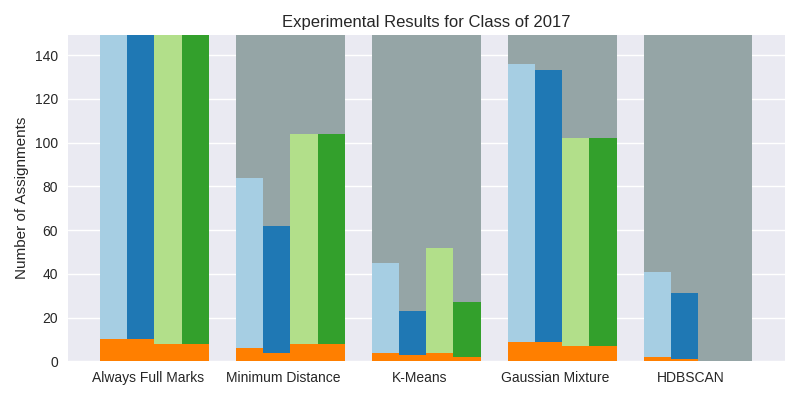
\includegraphics[width=\textwidth]{bar_triple_results_2017}
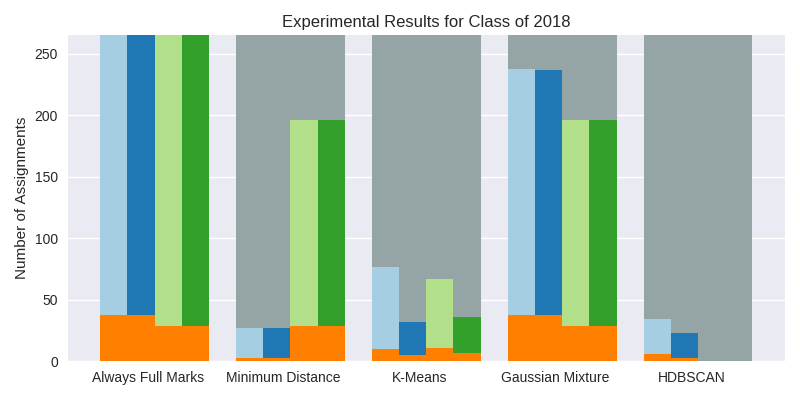
\includegraphics[width=\textwidth]{bar_triple_results_2018}
\caption[Experimental Results for Classes of 2017 and 2018]{These graphs break down the outcomes of the assignments for each class. The grey bars represent the number of assignments that must be manually marked; the light blue and dark blue bars represent the number of automated Non-Blocking IO assignments at the 90 and 95 cutoffs, respectively; similarly, the green bars represent the Parallel Processing assignment; and finally, the orange bars represent the number of automated assignments deemed to be false positives.}
\label{fig:ctm-results}
\end{figure}

Figure~\ref{fig:ctm-results} presents our experimental results. Since Always Full Marks did not perform any analysis, it would not encounter any processing errors and thus would always be able to automate every assignment. Clearly this was the maximum possible value and could not be exceeded; the goal for the other algorithms was to automate as many assignments as possible. While near-100\% automation rate was unrealistic due to potential processing errors, we hoped to be able to automate at least half the assignments. The false positives for Always Full Marks was simply the students that did not receive full marks. Therefore, we required the other algorithms to achieve a better false positive count than this trivial approach to be considered an improvement.

Firstly, the Minimum Distance algorithm was able to achieve slightly fewer false positives than Always Full Marks with an acceptable number of automated assignments. With the exception of Non-Blocking IO in 2018, this algorithm was able to automate almost half of the classes, which would greatly reduce the time needed for manual marking.

Secondly, the K-Means algorithm was able to achieve even fewer false positives than Minimum Distance; conversely, it automated even fewer assignments. However, we note that at the 90 cutoff, K-Means was still able to automate approximately a third of the assignments, which was a non-trivial reduction in manual work for human markers.

Thirdly, the Gaussian Mixture algorithm was able to achieve the highest automation rates out of all of our proposed algorithms. However, we note that this algorithm appeared to be strictly worse than the baseline Always Full Marks because its number of false positives was on par with the baseline despite not being able to automate as much.

Fourthly, the HDBSCAN algorithm was able to achieve the lowest number of false positives; conversely, it automated the fewest assignments. In addition, it appeared to be unable to flag any correct Parallel Processing solutions for the 2018 class; since this was exclusive to one class and not both, we believe this may have been due to minor assignment specification changes over the years and that our reference solutions were not up-to-date.

Finally, one common observation for all the graphs was that increasing the cutoff point decreased both the number of automated assignments and false positives. This was expected because a higher cutoff enforced a higher confidence in our prediction, i.e. the predicted score must be within 5 points of 100 to be considered correct instead of 10 points. Naturally, with a stricter requirement, the number of assignments that we could automate and the number of false positives also decreased.

\section{Shortcomings}

None of our proposed algorithms were able to achieve any meaningful reduction from Always Full Mark's number of false positives. As a result, we investigated potential sources of error that may have been been caused by our assumptions.

\subsection{Too Much Noise in Edit Distance}
\label{sec:ctm-too-much-noise}

One of the underlying assumptions that our tool made was that the edit distance we compute must accurately reflect the closeness of two program files. Although we tried encapsulating structural differences into a tree edit distance and ensuring logically similar code had low edit distances, the edit difference was still ultimately a scalar value that discarded potentially useful information.

When we manually inspected a couple of assignments marked as false positives (assignments that were automated to higher marks than they had earned from human markers), we noticed some of them had glaring issues that were not penalized as heavily relative to the overall edit distance. For example, one student did not use the Pthread library at all for the Parallel Processing assignment and thus should had failed. However, our tool only penalized  an edit distance of 100 for inserting the appropriate \texttt{CallStatement} nodes whereas final edit distances were normally between 500 to 800. As a result, this catastrophic failure went undetected as it got treated as a small outlier. This problem might had been caught if the penalty was magnitudes higher (e.g. \num{10000}). However, this might also obscure other issues because it would be magnitudes larger than other penalties.

Overall, we believe the single scalar value has too much noise to make accurate predictions. There are several avenues to pursue to improve this step: prune more unnecessary nodes from the ASTs, adjust the cost model penalties for key function calls, or generate a multi-dimensional matrix to represent program differences and to be used as input to our aggregator.

\subsection{Uncertain Ground-Truth}
\label{sec:ctm-uncertain-ground-truth}

There was some uncertainty in our ground-truth for the students' actual marks. Historical mark breakdowns were not archived and thus the marks we used include non-technical deductions such as issues with the student's written report, late submissions, or plagiarism. In addition, there was a discrepancy in marker leniency between the two years, as seen in Figure~\ref{fig:ctm-marker-discrepancy}. As a result, the \textquote{true} student marks that we used to measure our accuracy were not as reliable as we originally assumed.

\begin{figure}
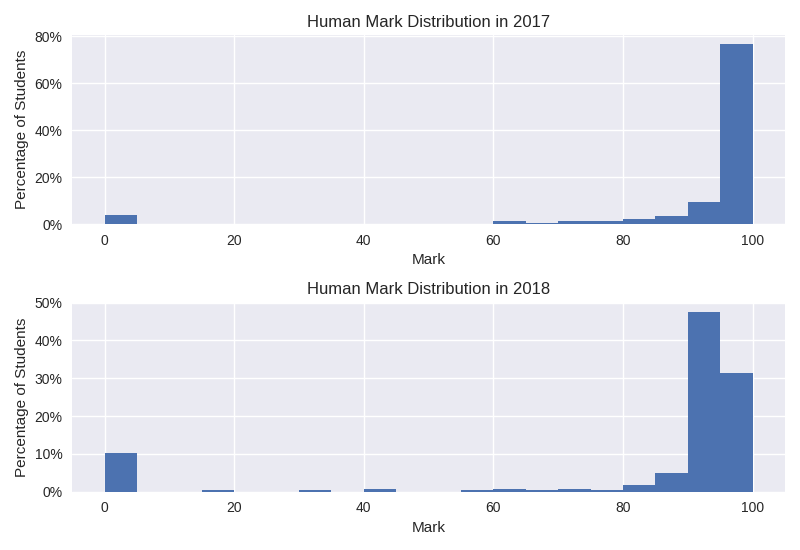
\includegraphics[width=\textwidth]{human_marks}
\caption[Marker Discrepancy Between 2017 and 2018]{There is a discrepancy in marker leniency between 2017 and 2018. Since markers change every semester, the two classes had different markers. In the 2017 class, about 80\% of the class received a 95 or higher from the marker whereas in the 2018 class, only 35\% of the class received a 95 or higher from the marker.}
\label{fig:ctm-marker-discrepancy}
\end{figure}

To verify whether the uncertainties in our ground-truth had a significant impact on our results in Section~\ref{sec:ctm-results}, we randomly selected 20 students from each class and remarked their assignments to ensure accuracy and consistency. Tables~\ref{tab:ctm-remarked-w2017} and \ref{tab:ctm-remarked-w2018} present the automation and false positive rates of our sampled students with their re-evaluated marks. Since we changed the ground-truth, only the false positive rate should change. However we still present the automation rate to verify that our random sample is representative of their entire class. This was indeed the case as we see that the automation rate was roughly identical to the automation rates of the entire class presented Figure~\ref{fig:ctm-results}; Gaussian Mixture had the highest automation rate while the others fell behind with HDBSCAN as the lowest.

When we compare the false positive rates, we see that Gaussian Mixture (the algorithm we initially observed to be strictly worse than the  baseline Always Full Marks) had a slightly better result than the baseline for both classes. In the 2017 class, Gaussian Mixture had zero false positives whereas the baseline had two false positives. Due to our small sample size and the fact that we were only able to automate 40\% of the students, this might had simply been a coincidence. However when we look at the 2018 class, we see that Gaussian Mixture was able to automate 70\% of the students with 21\% false positive rate compared to Always Full Marks at 35\% false positive rate.

Despite having a lower false positive rate than our baseline, 21\% is still too high to be considered usable in a live-classroom environment. Nonetheless, this sample has demonstrated promising potential in our tool to perform better than blindly assigning everyone full marks. Further refinements to our tool may eventually lead to a false positive rate low enough to be considered usable in a regular classroom.

\begin{table}
\caption{Automated Marks With New Ground-Truth for Class of 2017}
\label{tab:ctm-remarked-w2017}
\begin{tabular}{lrrrr} \toprule
\multirow{2}{*}{}
& \multicolumn{2}{c}{90 Cutoff} & \multicolumn{2}{c}{95 Cutoff}  \\
& Automated & False Positives & Automated & False Positives  \\
\midrule
Always Full Marks & 20 & 2 & 20 & 2 \\
Minimum Distance  & 5  & 0 & 5  & 0 \\
K-Means           & 2  & 0 & 2  & 0 \\
Gaussian Mixture  & 8  & 0 & 8  & 0 \\
HDBSCAN           & 0  & - & 0  & - \\
\bottomrule
\end{tabular}

\caption{Automated Marks With New Ground-Truth for Class of 2018}
\label{tab:ctm-remarked-w2018}
\begin{tabular}{lrrrr} \toprule
\multirow{2}{*}{}
& \multicolumn{2}{c}{90 Cutoff} & \multicolumn{2}{c}{95 Cutoff}  \\
& Automated & False Positives & Automated & False Positives  \\
\midrule
Always Full Marks & 20 & 7 & 20 & 7 \\
Minimum Distance  & 1  & 0 & 1  & 0 \\
K-Means           & 2  & 0 & 2  & 0 \\
Gaussian Mixture  & 14 & 3 & 14 & 3 \\
HDBSCAN           & 0  & - & 0  & - \\
\bottomrule
\end{tabular}
\end{table}

% Placing a * after \section means it will not show in the
% outline or table of contents.
\section*{Summary}

\begin{frame}{Summary}
\begin{itemize}

\item We presented a novel approach to automatically mark programming assignments

\item We demonstrated promising potential in using Gaussian Mixture clustering to aggregate AST TED into a final score
\begin{itemize}
\item Automate up to 70\% of assignments
\item Up to 21\% false positive rate vs. 35\% baseline
\end{itemize}

\end{itemize}
\end{frame}

\note{
\begin{itemize}
\item In summary, we've presented a novel approach to automatically mark programming assignments
\item We have demonstrated promising potential in using Gaussian Mixture clusting to aggregate AST edit distance into a final score
\item We've shown this can automate up to 70\% of the assignments with 21\% false positive rate, which is slightly better than our 35\% baseline
\item However, this is still too high to be usable in a live classroom. While no student would complain about getting more marks than they should have, a high false positive rate diminishes the value of assignments.
\end{itemize}
}

